\documentclass{standalone}
\author{Quinten Bruynseraede}
\usepackage{tikz}
\usetikzlibrary{shapes}
\title{Tikz grafen}
\begin{document}\pagestyle{empty}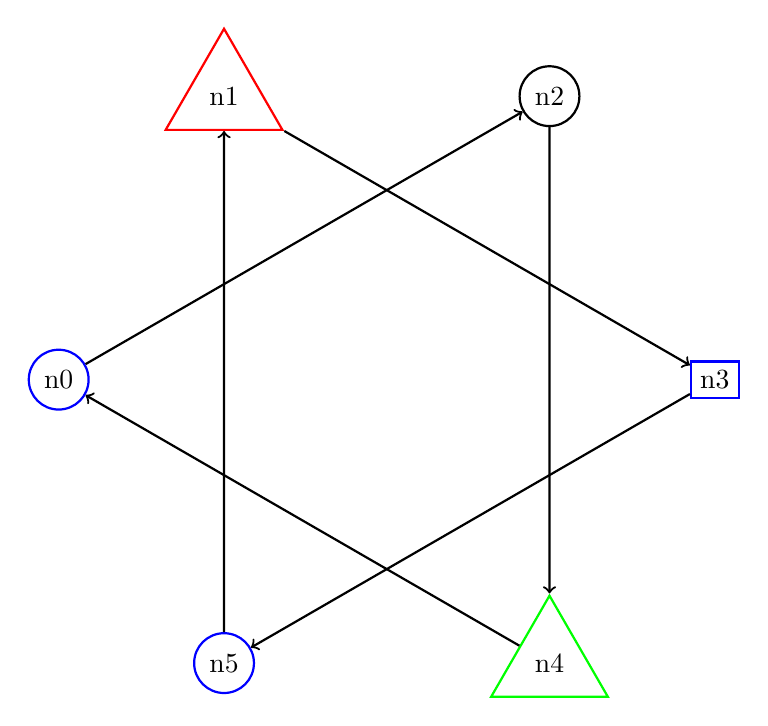
\begin{tikzpicture}\node[shape=circle,draw=blue,align=center,line width=0.8pt] (0) at (4.166666666666667,5.866666666666666) {n5};
\node[regular polygon,regular polygon sides=3,draw=green,align=center,line width=0.8pt] (1) at (8.3,5.866666666666666) {n4};
\node[shape=rectangle,draw=blue,align=center,line width=0.8pt] (2) at (10.4,9.466666666666667) {n3};
\node[shape=circle,draw=black,align=center,line width=0.8pt] (3) at (8.3,13.066666666666666) {n2};
\node[regular polygon,regular polygon sides=3,draw=red,align=center,line width=0.8pt] (4) at (4.166666666666667,13.066666666666666) {n1};
\node[shape=circle,draw=blue,align=center,line width=0.8pt] (5) at (2.066666666666667,9.466666666666667) {n0};

\path [->,draw=black,line width=0.8pt] (4) edge node {} (2);
\path [->,draw=black,line width=0.8pt] (3) edge node {} (1);
\path [->,draw=black,line width=0.8pt] (2) edge node {} (0);
\path [->,draw=black,line width=0.8pt] (1) edge node {} (5);
\path [->,draw=black,line width=0.8pt] (0) edge node {} (4);
\path [->,draw=black,line width=0.8pt] (5) edge node {} (3);
\end{tikzpicture}
\end{document}